\documentclass[10pt,aspectratio=169]{beamer}
\beamertemplatenavigationsymbolsempty
\usepackage{graphicx}
\usepackage{amsmath}
\usetheme{default}

\begin{document}
\begin{frame}
  \frametitle{What are we solving?}
  \begin{itemize}
    \item A system of 1D transport equations for tokamak plasmas.
    \item Evolves profiles of:
    \begin{itemize}
        \item Ion Temperature ($T_i$)
        \item Electron Temperature ($T_e$)
        \item Electron Density ($n_e$)
        \item Poloidal magnetic flux ($\psi$)
    \end{itemize}
    \item Self-consistently calculates:
    \begin{itemize}
        \item Plasma geometry
        \item Bootstrap current
        \item Conductivity
        \item Heating and particle sources
    \end{itemize}
  \end{itemize}
\end{frame}

\begin{frame}
  \frametitle{Core Physics Models}
  \begin{itemize}
    \item \textbf{Plasma Geometry:} The magnetic equilibrium (the shape of the nested magnetic surfaces) is determined by the plasma pressure and the total current profile.
    \item \textbf{Bootstrap Current:} A self-generated current driven by the plasma's pressure gradient in the toroidal geometry. It is essential for achieving efficient operation in a reactor.
    \item \textbf{Conductivity:} The plasma's ability to carry current, which is the inverse of resistivity. It strongly on the electron temperature and the amount of impurities in the plasma ($Z_{eff}$).
    \item \textbf{Heating and Particle Sources:} These are user-defined profiles that model the injection of energy and particles that sustain the plasma.
  \end{itemize}
\end{frame}

\begin{frame}
  \frametitle{Numerical Scheme}
  \begin{itemize}
    \item \textbf{PDEs:} 1D (in $\rho$) coupled, nonlinear, second-order parabolic transport equations.
    \item \textbf{Spatial Discretization:} Finite Volume Method on a staggered grid.
    \begin{itemize}
        \item Diffusion: Central differencing.
        \item Convection: Upwind scheme with a Peclet number-dependent flux limiter.
    \end{itemize}
    \item \textbf{Boundary Conditions:}
    \begin{itemize}
        \item Core ($\rho=0$): Zero-gradient (Neumann).
        \item Edge ($\rho=1$): Fixed value (Dirichlet).
    \end{itemize}
    \item \textbf{Time Stepping:} Fully implicit backward Euler method.
    \begin{itemize}
        \item A predictor-corrector or Newton-Raphson method solves the nonlinear system.
    \end{itemize}
    \item \textbf{Coefficients \& Sources:} Self-consistently calculated from physics models (e.g., QLKNN, Sauter).
  \end{itemize}
\end{frame}

\begin{frame}[plain]
  \begin{figure}
    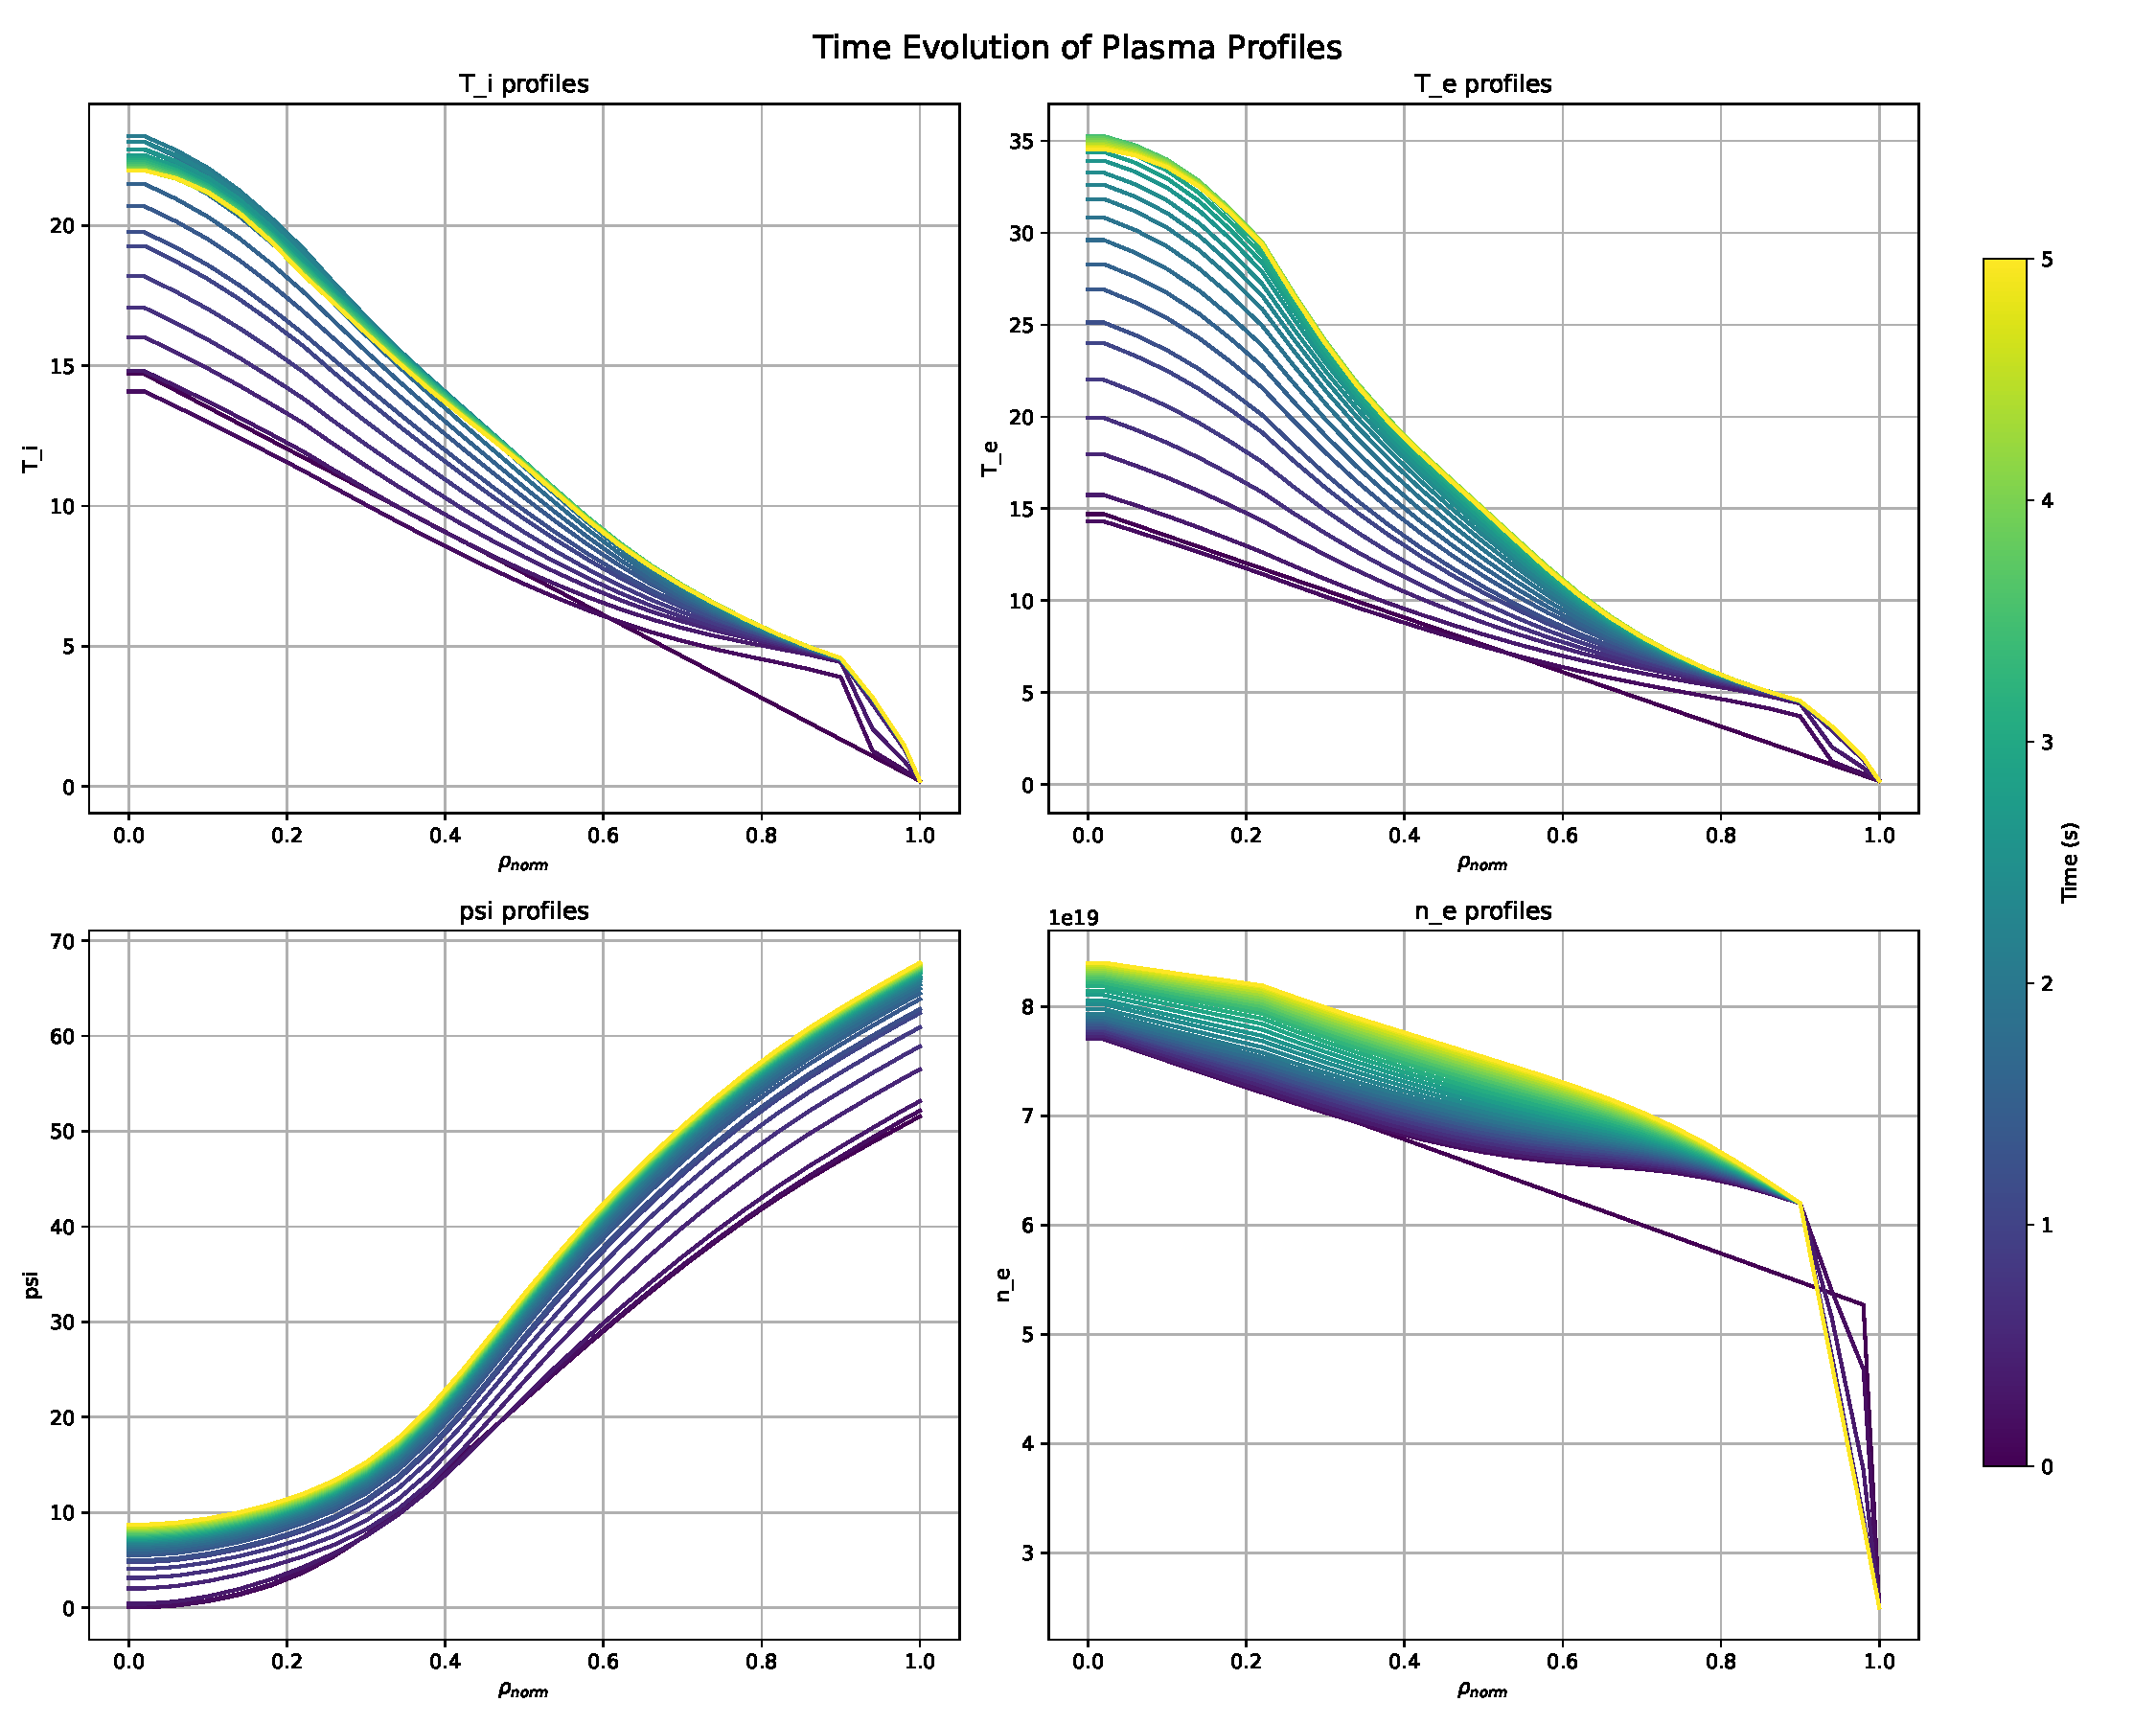
\includegraphics[width=0.8\textwidth]{all_profiles.pdf}
  \end{figure}
\end{frame}

\begin{frame}[allowframebreaks]
  \bibliographystyle{abbrv}
  \bibliography{main}
  \nocite{*}
\end{frame}

\end{document}
